% LaTex file for Stephen Balakirsky's RITA 2014 submission
%
\documentclass{llncs}
%
\usepackage{makeidx}  % allows for indexgeneration
%
% my additional packages
\usepackage{graphicx}
\usepackage{multirow,array}
\usepackage{rotating} % for sideways
\usepackage{amsmath}
\usepackage{amsthm}
%\usepackage{algorithm2e}
\usepackage[linesnumbered, boxed, figure]{algorithm2e}
%
% zeid's definitions
\newcommand{\class}[1] {\textit{#1}}
\newcommand{\const}[1] {$\mathit{#1}$}
\newcommand{\objvar}[1] {$\mathsf{#1}$}
\newcommand{\stvar}[1] {\textsf{#1}}
%
%
\begin{document}
%
\frontmatter          % for the preliminaries
%
\pagestyle{headings}  % switches on printing of running heads
\addtocmark{Hamiltonian Mechanics} % additional mark in the TOC
%
%
\mainmatter              % start of the contributions
%
\title{An Ontology Based Approach to Action Verification for Agile Manufacturing}
%
\titlerunning{Agile Manufacturing}  % abbreviated title (for running head)
%                                     also used for the TOC unless
%                                     \toctitle is used
%
\author{Stephen Balakirsky\inst{1} \and Zeid Kootbally\inst{2}}
%
\authorrunning{Stephen Balakirsky et al.} % abbreviated author list (for running head)
%
%%%% list of authors for the TOC (use if author list has to be modified)
\tocauthor{Stephen Balakirsky, Zeid Kootbally}
%
\institute{Georgia Tech Research Institute, Atlanta, GA 30332, USA,\\
\email{stephen.balakirsky@gtri.gatech.edu},\\ WWW home page:
\texttt{unmannedsystems.gtri.gatech.edu}
\and
University of Maryland, College Park, MD 20740, USA,\\
\email{zeid.kootbally@umd.edu},\\ WWW home page:
\texttt{www.nist.gov/el/isd/ks/kootbally.cfm}
}

\maketitle              % typeset the title of the contribution

\begin{abstract}
Many of today’s robotic workcells are unable to detect when an action failure has occurred. This results in faulty products being sent down the line, and/or downtime for the cell as failures are detected and corrected. This article examines a novel knowledge-driven system that provides added agility by detecting and correcting action failures. The system also provides for late binding of action parameters, thus providing flexibility by allowing plans to adapt to changing environmental conditions. The key feature to this system is its knowledgebase that contains the necessary relationships and representations to allow for the failure detection and correction. This article presents the ontology that stores this knowledge as well as the overall system architecture. The manufacturing domain of kit construction is examined as a sample test environment. 
\end{abstract}
%
%
\section{Introduction}
A failure is any change, design, or manufacturing error that renders a component, assembly, or system incapable of performing its intended function \cite{Collins93}. In kitting, as described in Section \ref{sect:kitting}, failures can occur for multiple reasons that include equipment not being set up properly, tools and/or fixtures not being properly prepared, and improper equipment maintenance. Part/component availability failures can be triggered by inaccurate information on the location of the part, part damage, incorrect part types, or part shortage due to delays in internal logistics. In order to prevent or minimize failures, a disciplined approach needs to be implemented to identify the different ways a process design can fail before impacting productivity.

Even though today's state-of-the-art industrial robots are capable of sub-millimeter accuracy \cite{RobotAccuracy}, they often lack the sensing
necessary to detect failures and the programming required to cope with and correct the failure. This is due to the fact that they are often programmed
by an operator using crude positional controls from a teach pendant. These teach pendant programs are highly repeatable, which provides 
utility for large-batch, error-free operation. However, the cyclic program that repeats identical operations does not lend itself well to adaptation for 
failure mitigation. In fact, producing a program to correct a perceived failure would require that the cell be taken off-line
for additional human-led teach pendant programming. In addition, 
most cells lack the ability to sense that a failure occurred and  lack programming (that would have had to be teach pendant entered) to cope
with failure conditions, thus making it impossible for the cell to recover from failures.
This leads to faulty products being sent down the line, and/or downtime for the cell as failures are detected and corrected.

For small batch processors or other customers who must frequently change their line configuration or desire to perform complex operations
with their robots, this frequent downtime and lack of failure correction/detection may be unacceptable. The robotic systems of tomorrow need to be capable, flexible, and agile.  
These systems need to perform their duties at least  as well as human counterparts, be quickly re-tasked to other operations, cope with a wide 
variety of unexpected environmental and operational changes, and be able to detect and correct errors in operation. 
To be successful, these systems need to combine domain expertise, knowledge of their own skills and limitations, and both semantic and geometric 
environmental information.

The IEEE Robotics and Automation Society's Ontologies for Robotics and Automation Working Group has taken the first steps in creating the 
infrastructure necessary for such a system, while the Industrial Subgroup has applied this infrastructure to create a sample kit building
system.  This work is presented in Balakirsky et al. \cite{balakirsky2013} which describes the construction of a robotic kit building
system that is able to cope with environmental and task changes without operator intervention. This article extends that work to utilize
the same infrastructure to allow for the detection and correction of action failures in the system.

The organization of the remainder of this paper is as follows. Section \ref{sect:kitting} describes the domain of kit building. Section \ref{sect:overview} presents
an overview of the software system architecture as well as details of the ontology and world model for the robot cell. Section \ref{sect:operation} discusses the detailed operation of cell, and Section \ref{sect:failure} discusses how failures are handled by the ontology. Finally, Section \ref{sect:future} presents
conclusions and future work.
%
%
\section{Kitting}
\label{sect:kitting}
Today's advanced manufacturing plants utilize mixed-model assembly where multiple product variants are built on the same line.  
According to Jim Tetreault, Ford’s vice president of North America Manufacturing, 
new Ford assembly facilities are able to build a full spectrum of vehicles on the same assembly line \cite{James2011}. One of the technologies that makes this possible
is the use of assembly kits.  Bozer and McGinnis \cite{Bozer1992} describe a kit as ``a specific
collection of components and/or subassemblies that together (i.e., in the same container) support one or more assembly
operations for a given product or shop order''. These  kits provide a synchronous material flow, where parts and components move to 
assembly stations in a just-in-time manner. The kits provide workers with the parts and tools that they need (which may vary from 
vehicle model to vehicle model) in the sequence that they need them. The use of kitting also allows a single delivery system to feed
multiple assembly stations thus saving manufacturing or assembly space \cite{Medbo2003} and provides an additional inspection opportunity 
that allows for the detection of part defects before they impact assembly operations. The individual operations of the station 
that builds the kits may be viewed as a specialization of the general
bin-picking problem \cite{Schyja2012} where parts are picked from one or more part bins or trays and placed into specific slots in a kit tray.

For our sample implementation, we assume that the robot cell is building one of several possible kit configurations. At execution time, the
cell has a set kit to build, but does not know the precise location of the kit tray, the part trays, or the location of individual parts in the part tray.
When a human builds a kit, they are able to inspect each part before adding it to the kit tray. This provides an additional level of quality control and
is an aspect that is desirable to have in our robotic system. During kit construction,
a robot performs a series of pick-and-place operations
in order to construct the kit. These operations include:
\begin{enumerate}
\item Pick up an empty kit and place it on the work table.
\item Pick up multiple component parts, inspect them, and place them in the kit.
\item Pick up the completed kit and place it in the full kit storage area.
\end{enumerate}
Each of these steps may be a compound action that includes
other actions such as end-of-arm tool changes, path planning,
and obstacle avoidance. The items that are being placed in the kit may be of varying size and shape and have various grasping and inspection
requirements.
%
\begin{figure}[htb!]
\begin{center}
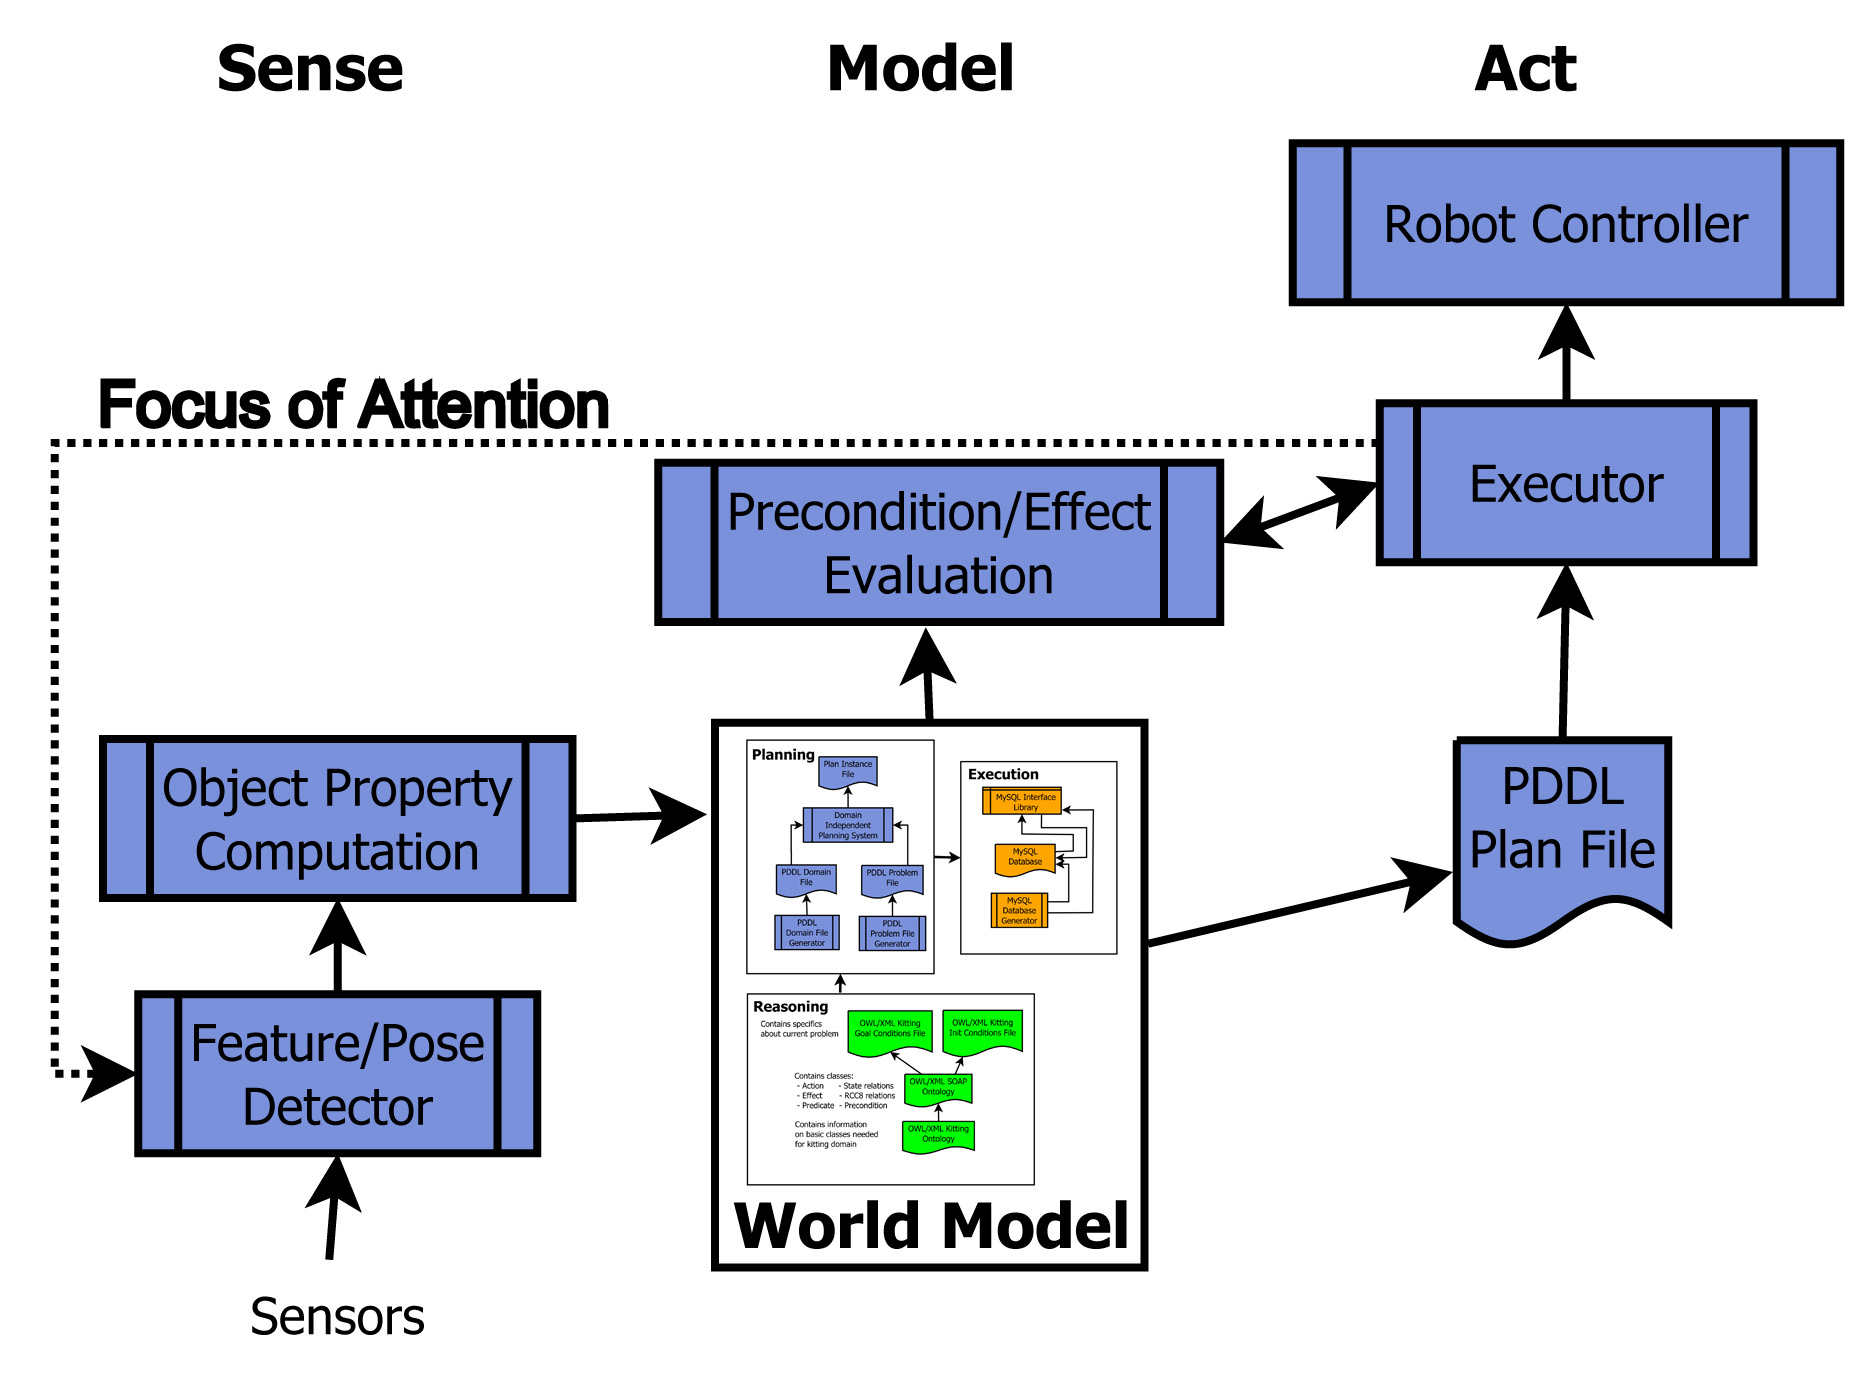
\includegraphics[width=8.5cm]{images/RITAExecution.jpg}
\caption{Major components that make up the Sense--Model--Act paradigm of the kitting station.}
\label{fig:SenseModelAct}
\end{center}
\end{figure}
\section{System Overview}
\label{sect:overview}
The kitting system that has been implemented as part of this work is a deliberative intelligent system based on the 4D/RCS 
reference model architecture \cite{Albus2000}. This architecture is a hierarchical architecture in which each echelon or level
follows a sense-model-act paradigm. The basic structure of the system may be seen in Figure \ref{fig:SenseModelAct}.
%
\subsection{Sense}
\label{subsection:Sense}
In order to sense action failures associated with kit building, it is necessary to be able to detect the six-degree of freedom pose of relevant objects in the
world. One issue with pose detection is the large number of potential target objects and object classes in the world. 
Both the number of objects and potential classes can be reduced by intelligently
selecting critical objects of interest that are tagged with predicted locations and object classes for the sensor system to track. This object selection, 
also known as focus of attention, is guided by
the executor process with knowledge obtained from preconditions and effects of planned actions.
Actual algorithm development for pose and object detection is an active research area, and is beyond the scope of this article. 

For our purposes, 
we have assumed the use of a high-quality
system that is capable of recognizing a limited variety of items in a controlled environment and then determining the item's pose. This is accomplished through
simulation by using the Unified System for Automation and Robot Simulation (USARSim) \cite{Balakirsky2007}. As described in Section \ref{sect:future}, 
we intend to relax this assumption in the near future.
%
\begin{figure}[htb!]
\begin{center}
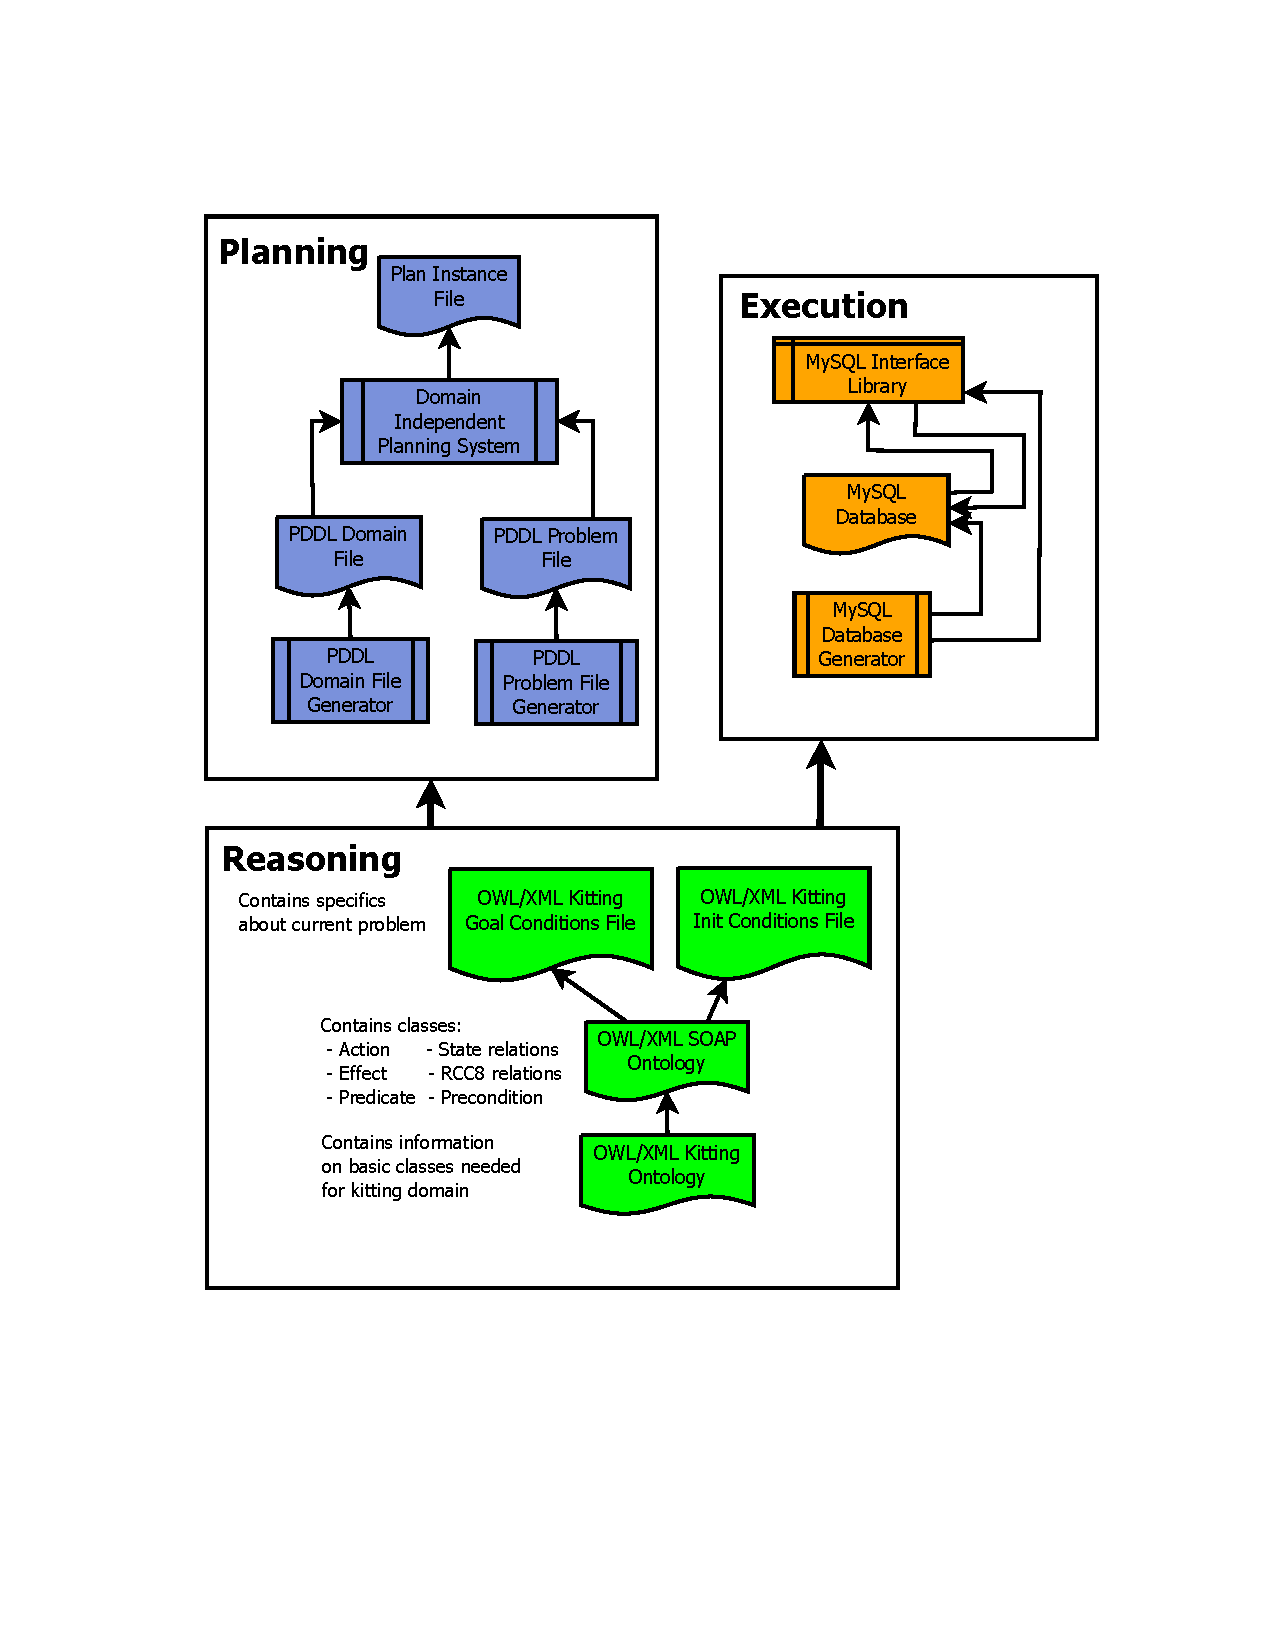
\includegraphics[width=8.5cm]{images/RITAWorldModel.pdf}
\caption{System World Model - The world model contains an ontology shown in green,
a Planning Domain Definition Language (PDDL) specification shown in blue, and a dynamic database shown in orange.}
\label{fig:WorldModel}
\end{center}
\end{figure}
%
\subsection{Model}
\label{subsection:Model}
The world model that is being utilized is shown in Figure \ref{fig:WorldModel}. The model contains knowledge that is structured specifically for
reasoning, planning, and execution. All of the concepts necessary for the manufacturing domain under test are
encoded in the ontology that resides in the reasoning section of the model. The planning and execution sections of the model are automatically generated from
this section.
%
\subsubsection{Ontology --}
\label{sect:Ontology}
The reasoning portion of the world model is designed to contain all of the information needed to reason over and solve complex manufacturing
problems. The knowledge is represented in an ontology that is structured in three parts. The first part of the ontology is an upper ontology
that contains generic information and classes that are needed for the domain of kit building. 

This area of the ontology contains information on basic elements such as a ``point" which is defined as a class that contains a name 
and a three-dimensional quantity, as well as complex types such as a ``part'', which is
shown in Figure \ref{fig:part}, and
contains elements such as a the part's shape, stock keeping unit (SKU) number, and location. This information is utilized to create parameters for the Planning World
Model and the skeleton tables for the MySQL database of the Execution World Model.
%
\begin{figure}[htb!]
\begin{center}
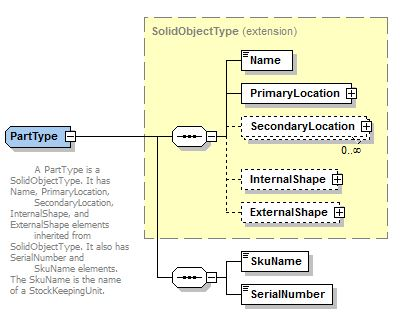
\includegraphics[width=8.5cm]{images/Part.jpg}
\caption{Description of the PartType class that is designed to contain both static and dynamic information about particular parts.}
\label{fig:part}
\end{center}
\end{figure}
%
Both static and dynamic information is represented in this
ontology and is automatically transitioned into the Planning and Execution areas of the world model. During system
operation,  dynamic information is updated in the Execution World Model.
More information on this portion of the ontology may be found in \cite{Balakirsky2012-1}.


The second part of the ontology (known as States, Ordering constraints, Actions, and Predicates or SOAP) contains the high-level concept of an action and all of the concepts 
that are required to support an action. In this case, a Planning Domain Definition Language (PDDL) \cite{PDDL} action is being represented, and this action is defined
 as an operator that causes one or more properties of an 
instance to change. Before this action may be
performed, certain preconditions must be satisfied, and after the action is performed, certain effects will take place. The action accepts parameters that specify the particular
instances that will be affected, where an instance refers to a physical object in the world. The classes used to represent the actions in the ontology are provided in the
enumerated list shown below. The naming convention utilized follows the OWL \cite{OWLoverview} implementation of the ontology.

ZEID, FIX HERE!

\begin{enumerate}
\item \class{Action} -- An \class{Action} has an \class{ActionPrecondition} and an \class{ActionEffect}. An \class{Action} has an \class{ActionParameterList} that contains all the parameters for an action. An \class{Action} has a unique name.
\item \class{ActionParameterList} -- Actions may have multiple parameters of different types. Each one of these types is represented by a class in the upper ontology. The \class{ActionParameterList} has parameters (\emph{hasActionParameter}) that are instances from the upper ontology. The order of the parameters in an  action also needs to be represented in the ontology. OWL has no built-in structure to represent an ordered list, instead, the parameter, uses \emph{hasNextParameter} and \emph{hasPreviousParameter} to point to the next and the previous parameter in \class{ParameterList}, respectively.
\item \class{ActionPrecondition} -- An \class{ActionPrecondition} can consist of an \class{ActionPredicate}, an \class{ActionFunction}, an \class{ActionFunctionBool}, or a combination of these three classes. An \class{ActionPrecondition} belongs to one \class{Action}.
\item \class{ActionEffect} -- An \class{ActionEffect} can consist of an \class{ActionPredicate}, an \class{ActionFunction}, an \class{ActionFunctionBool}, or a combination of these three classes. An \class{ActionEffect} belongs to one \class{Action}. A negative \class{ActionPredicate} is represented with the declaration of \emph{hasEffect\_Predicate} within the OWL built-in property assertion \texttt{owl:NegativePropertyAssertion}.
\item \class{ActionPredicate} -- An \class{ActionPredicate} has a unique name of type \texttt{string}. An \class{ActionPredicate} has a reference parameter and a target parameter. A reference parameter is the first parameter in the parameter's list and the target parameter is the second parameter in the parameter's list. An \class{ActionPredicate} cannot have more than two parameters due to the inherent definition of predicates. In the case where an \class{ActionPredicate} has only one parameter, it is assigned to the reference parameter. Reference and target parameters are one of the parameters defined for the \class{Action} to which the \class{ActionPredicate} belongs.


The meaning of reference and target parameters lies in the definition of a state variable. We recall the following definition of a state variable\\ $\mathrm{x: A_1\times \dots\times A_i\times S\rightarrow B_1\cup\dots\cup B_j}$ ($i, j\geq 1$) that is used to convert state variables into predicates as follows:

\begin{itemize}
 \item $\mathrm{A_1\times \dots\times A_i\times S\rightarrow B_1\cup\dots\cup B_j}$ ($i, j\geq 1$)
  \begin{itemize}
  \item \stvar{predicate\_1}($\mathcal{A,B}$)
  \item \ldots
  \item \stvar{predicate\_n}($\mathcal{A,B}$)
  \end{itemize}
\end{itemize}

Where $\mathcal{A} \in \mathrm{\{A_1,\ldots,A_i\}}$ and $\mathcal{B} \in \mathrm{\{B_1,\ldots,B_i\}}$ ($i, j\geq 1$)

From this methodology, we have defined a predicate's parameter as a reference parameter if the parameter belongs to the set $\mathcal{A}$. Similarly, we have defined a predicate's parameter as a target parameter if the parameter belongs to the set $\mathcal{B}$. For instance, the predicate \texttt{(part-location-robot ?part ?robot)} has \texttt{?part} as the reference parameter and \texttt{?robot} as the target parameter. This convention has been used in our ontology to define these two distinct types of parameters.

\item \class{ActionFunction} -- An \class{ActionFunction} has a unique name  of type \texttt{string}. An \class{ActionFunction} has a reference parameter and a target parameter. The same rules apply to the definition and use of these two types of parameters as the ones defined for \class{ActionPredicate}.
\item \class{ActionFunctionBool} -- \class{ActionFunctionBool} has one or more subclasses that represent the type of relation (mathematical operator) between two \class{ActionFunction}s. Subclasses of \class{ActionFunctionBool} have a first \class{ActionFunction} that represents the \class{ActionFunction} on the left side of the operator. Subclasses of \class{ActionFunctionBool} have a second \class{ActionFunction} that represents the \class{ActionFunction} on the right side of the operator.
\end{enumerate}

The third part of the ontology contains specific instances needed for a particular kitting domain. For example, it will contain the definition of the finished kits that may be
constructed and specific information on the individual parts. One of the goals of this framework is to introduce additional agility into the kit building process. Therefore,
partial information is accepted and even encouraged for this area of the ontology. For the example of a part shown in Figure \ref{fig:part}, information on the SKU, grasp points 
(part of the ExternalShape or InternalShape), and name would be expected to be available at runtime. Information on the location of the part (PrimaryLocation) may not
become valid until after a sensor processing system has identified and located the particular part.
%
\subsubsection{Planning --}
The Planning Domain Definition Language (PDDL)  is an attempt by the domain independent planning community to formulate a standard language for planning. A community of planning researchers has been producing planning systems that comply with this formalism since the first International Planning Competition held in 1998. This competition series
continues today, with the seventh competition being held in 2011. PDDL is constantly adding extensions to the base language in order to represent more expressive problem domains. The representation in the world model is based on PDDL Version 3.

By placing the knowledge in a PDDL representation, the use of an entire family of open source planning systems such as the forward-chaining partial-order planning system from Coles et al. \cite{Coles.ICAPS.2010}
is enabled. In order to operate, the PDDL planners require a PDDL file-set that consists of two files that specify the domain and the problem.
From these files, the planning system creates an additional static plan file.

This plan file contains a sequence of actions that will transition the system from the initial state to the goal state. In order to maintain flexibility, it is desired that detailed information that is subject to change should be ``late-bound'' to the plan. In other words, specific information is acquired directly before that information needs to be used by the system. This allows for last minute changes in this information. For example, the location of a kit tray on a work table may be different from run to run. However, one would like to be able to use the same planning sequence for constructing the kit independent of the tray's exact position.
To compensate for this lack of exact knowledge, the plans that are generated by the PDDL planning system contain only high-level actions.

As seen in Figure \ref{fig:WorldModel}, the planning world model framework contains generators that read the ontology and create
a standard PDDL domain and PDDL problem file. Any of the family of PDDL Version 3 compatible planning systems is then able to be
run on these files to create the static plan instance file. A representation of this plan may be stored in the ontology for future use.
%
\subsubsection{Execution --}
The execution world model is also built automatically from the ontology. This world model consists of a MySQL database and C++ and Java
interfaces that provide for easy access to the data. The table skeletons are generated from the kitting ontology, and the tables are initially populated
with information from the initial and goal condition files. During plan execution, the executor guides the sensor processing system
in updating the information in 
this section of the world model. All of the data structures encoded in the ontology are included in this representation. 
%An example 
%of the data tables that are created may be seen in Figure ?? for the Part class that is shown in Figure \ref{fig:part}. 
%
\subsection{Act}
\label{subsection:Act}
The actions that take place in the kitting work cell are coordinated by the Executor as illustrated in Figure \ref{fig:SenseModelAct}.  The Executor
reads PDDL actions as input and outputs a standardized set of low-level robot commands developed at the National Institute of Standards
and Technology (NIST) known as the  Canonical Robotic Control Language \cite{Balakirsky2012-1}. 

Before and after each high-level command
is executed, the Executor sends focus of attention information into the sensor processing system. This allows the sensor processing system to compute
the appropriate predicate relations that are required to verify the conditions necessary to carry out an action and that an action's execution has
been successful. Information on predicates is written to the world model by the sensing system and read from the world model by the executor.
%
\\
\begin{algorithm}[h!]

 \KwData{ $kitToBuild$ }
 \KwResult{reports success or failure}
 	retrieve instance $PDDLInstance$ to construct kit $kitToBuild$\;
 	\For{each action $\textbf{A}$ in $PDDLInstance$}{
 		\For{each precondition $\textbf{P}$ of action $\textbf{A}$} {
			\If{$PredicateEvaluation(P)=false$}{
				report failure\;
			}
 		}
 		create set $S$ of Canonical Robot Control Language Commands\;
 		send set $S$ to Robot Controller for execution\;
 		\For{each effect $\textbf{E}$ of action $\textbf{A}$} {
			\If{$PredicateEvaluation(E)==false$}{
				report failure\;
			}
 		}
 		report action success\;
 	}
 	report plan success\;
\caption{{\sc BuildKit} -- Sequences the actions necessary to build a kit.}
\label{fig:buildkit}
\end{algorithm}
%
\section{System Operation}
\label{sect:operation}
In order to construct a kit, the kitting system steps through each action in
the precomputed PDDL plan. Failures are searched for both before and after execution of 
each action. The overall process, known as {\sc BuildKit} is shown in Figure
\ref{fig:buildkit}. 

This process begins by retrieving a planning instance that has been 
precomputed to solve the construction of the requested kit (Line 1 of 
Figure \ref{fig:buildkit}). This is a high-level PDDL
plan that is not grounded to actual part instances or locations. It contains information
on the named storage location for classes of parts (individual SKU numbers), 
the quantity of each SKU that is required by the kit, and a build order (a sequence
of SKUs to be added to the kit). Additional information on the appropriate
end-of-arm tooling required to grip each part is also included.

This planning instance is decomposed into individual actions that must
be successfully carried out to complete the construction of the kit (the
{\it for} loop beginning at Line 2 of Figure \ref{fig:buildkit}). At this point,
preconditions of the action are examined to assure that the action to be attempted
is valid. If any of the action's preconditions are not able to be validated,
a failure is reported; otherwise, the action is approved for execution.
%
\begin{algorithm}[h!]
 \KwData{ $PredicateIn$ }
 \KwResult{true or false}
 	determine predicted pose $PoseR$ of $PredicateIn.ReferenceParameter$
 	and $PoseT$ of $PredicateIn.TargetParameter$ \;
 	send $PredicateIn$, pose $PoseR$, and $PoseT$ as focus of attention command to $SensorProcessing$\;
   	\uIf{$Eval(PredicateIn) == true$}{
 		return true\;
 	}
 	\Else{
 		return false \;
 	}
\caption{{\sc PredicateEvaluation} -- Returns the truth value of the predicate expression.}
\label{fig:predicateEval}
\end{algorithm}
%
\subsection{Precondition Validation}
\label{sect:preconditionValid}
Each precondition is a predicate expression that must be validated prior to
action execution.
The procedure for validating predicates is shown in Figure \ref{fig:predicateEval}. In Line 1 of this algorithm, the world
model is queried for the pose and class of each relevant 
parameter of the predicate. The information returned is the 
latest knowledge that has been recorded by the sensor processing
system and is not guaranteed to be up-to-date. This predicted
knowledge is sent as a focus of attention indicator to the sensor
processing system, and the sensor processing system is instructed to
update the predictions in the world model with current observations
and to compute the supporting relationships necessary for predicate
evaluation.
%
\begin{algorithm}[h!]
 \KwData{ $PredicateIn, PoseR, PoseT$ }
 	determine actual pose $APoseR$ of $PredicateIn.ReferenceParameter$\;
 	determine actual pose $APoseT$ of $PredicateIn.TargetParameter$\;
 	determine RCC8 relations between $APoseR$ and $APoseT$\;
 	determine Intermediate State Relations based on RCC8 relations\;
 	determine truth value of $PredicateIn$ and write to MySQL database\;
\caption{{\sc SensorProcessing} -- Updates the MySQL database in the Execution world model
to contain the latest evaluation of predicates related to $PredicateIn$.}
\label{fig:sensorProcess}
\end{algorithm}
%
Figure \ref{fig:sensorProcess} depicts the algorithm that is followed by
sensor processing in the computation of predicate values. As may be seen from this
figure, the computation of predicates is a three step process that involves
the computation of increasingly complex forms of spatial relations. These
relationships; Region Connection Calculus (RCC8) relations, intermediate state relations, and predicate relations, are each represented as a separate class in
the ontology.
%
\subsubsection{RCC8 Relation --}
RCC8 \cite{Wolter2000} is an approach for representing the relationship between two regions in Euclidean or topological space. The class \class{RCC8\_Relation} 
is based on the definition of RCC8 and consists of eight possible relations that include Tangential Proper Part (TPP), Non-Tangential Proper Part(NTPP), Disconnected (DC), Tangential Proper Part Inverse (TPPi), Non-Tangential Proper Part Inverse (NTPPi), Externally Connected (EC), Equal (EQ), and Partially Overlapping (PO). In order to represent these relations in all three dimensions for the kitting domain, RCC8 has been extended to a three-dimensional space by applying it along all three planes (x-y, x-z, y-z) and by including cardinal direction relations ``+'' and ``-''. In the ontology, RCC8 relations and cardinal direction relations are represented as subclasses of the class \class{RCC8\_Relation}. 
%
\subsubsection{Intermediate State Relation --}
These relations can be inferred from the combination of RCC8 and cardinal direction relations. For  instance, the intermediate state relation \textbf{In-Contact-With} is used to describe that object \textit{obj1} is in contact with object \textit{obj2}. This is true if \textit{obj1} is externally connected to \textit{obj2} in the x-direction, the y-direction, or the z-direction,  and is represented with the following combination of RCC8 relations:
\begin{gather}
\textbf{In-Contact-With}(\textit{obj1}, \textit{obj2}) \rightarrow   \notag\\
\texttt{x-EC}(\textit{obj1}, \textit{obj2}) \vee \texttt{y-EC}(\textit{obj1}, \textit{obj2}) \vee \texttt{z-EC}(\textit{obj1},\textit{obj2}) \notag
\end{gather}
In the ontology, intermediate state relations are represented with the OWL built-in property \texttt{owl:equivalentClass} that links the description of the class \class{Intermediate\_State\_Relation} to a logical expression based on RCC8 relations from the class \class{RCC8\_Relation}.
\subsubsection{Predicate Relation --} The truth-value of predicates can be determined through the logical combination of intermediate state relations. The predicate \class{endeffector-location-endeffectorholder}(\textit{endeffector}, \textit{endeffectorholder}) is true if and only if the location of the end effector \textit{endeffector} is in the end effector holder \textit{endeffectorholder} and is not attached to a robot. This predicate can be described using the following combination of intermediate state relations:
\begin{gather}
\textsf{endeffector-location-endeffectorholder}(\textit{endeffector},\textit{endeffectorholder}) \rightarrow   \notag\\
\textbf{In-Contact-With}(\textit{endeffector}, \textit{enfectorholder}) \wedge \notag\\
\neg\textbf{In-Contact-With}(\textit{endeffector}, \textit{robot}) \notag
\end{gather}
As with state relations, the truth-value of predicates is captured in the ontology using the \texttt{owl:equivalentClass} property that links the description of the class \class{Predicate} to the logical combination of intermediate state relations from the class \class{Intermediate\_State\_Relation}.
\subsubsection{Truth Value Determination --}
As seen in Section \ref{sect:Ontology}, a predicate can have a maximum of two parameters. In the case where a predicate has two parameters, the parameters are passed to the intermediate state relations defined for the predicate, and are in turn passed to the RCC8 relations were the truth-value of these relations are computed. In the case the predicate has only one parameter, the truth-value of intermediate state relations, and by inference, the truth-value of RCC8 relations will be tested with this parameter and with every object in the environment in lieu of the second parameter. Our kitting domain consists of only one predicate that has no parameters. This predicate is used as a flag in order to force some actions to come before others during the formulation of the plan. Predicates of this nature are not treated in the concept of ``Spatial Relation''.

These truth values may be retrieved from the ontology for use in Line 3 of Figure
\ref{fig:predicateEval} which will then propagate back up to {\sc BuildKit}. If
the predicates are successfully evaluated, the action will be cleared for 
execution and a set of CRCL Commands will be 
generated.
%
\begin{figure}[htb!]
\begin{center}
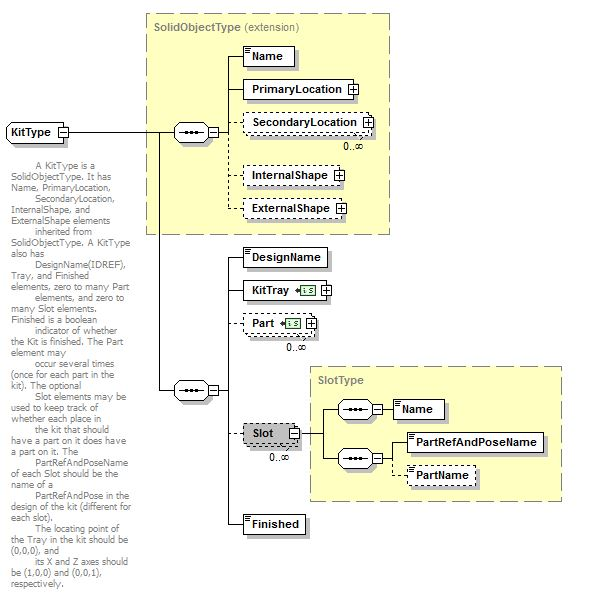
\includegraphics[width=12cm]{images/Kit.jpg}
\caption{Description of the KitType class that is designed to bring together
a container (the KitTray), a design for the kit creation, and specific parts
that populate the kit.}
\label{fig:kit}
\end{center}
\end{figure}
%
\subsection{Canonical Robot Control Language Generation}
Up to this point, the PDDL actions are not fully grounded to specific instances
that exist in the world. For example, the action \texttt{put-part} is designed
to place the part that is currently being held by the robot into a kit that
is specified as one of the action's input parameters. However, the precise
location for this part to be placed is not specified at the time of plan
creation. It is up to the Executor, working with the world model, to find
an empty slot in the kit that can receive the part. The structure of the
ontology is specifically designed to support this grounding, and this
structure is automatically replicated in the MySQL database that resides
in the Execution portion of the world model. 

Continuing with
the example of the \texttt{put-part} command, the Executor needs to find
an empty slot in the target kit to place the specific part that the robot is
holding. As shown in Figure \ref{fig:kit}, the {\sc KitType} class contains
zero to many {\sc Slot} classes that in turn contain specific location and 
part identification information. The Executor is able to read this information
from the world model and determine the precise global pose where the part
should be placed. The robot controller must now be commanded to complete this action.

While the action is an atomic element in PDDL, it will decompose into a series
of actions in CRCL. The robot will need to follow a safe trajectory to achieve
the slot in the kit, and the gripper will need to be controlled in order to release
the part. This one-to-many mapping is performed in the Executor and is currently
hand-coded for each of the PDDL commands that exists in the system. 
%
\subsection{Effect Validation}
The purpose of performing an action is to achieve results in the world. These results are represented in the PDDL effects. Each effect is a predicate expression that must be validated to assure proper
action execution. The technique for validating the effect predicates is identical
to the evaluation of the precondition predicates described in Section \ref{sect:preconditionValid}. If all of the effects are able to be validated, the
system will report the action's success and begin performing the next action in the plan.
%
\begin{figure}[htb!]
\begin{center}
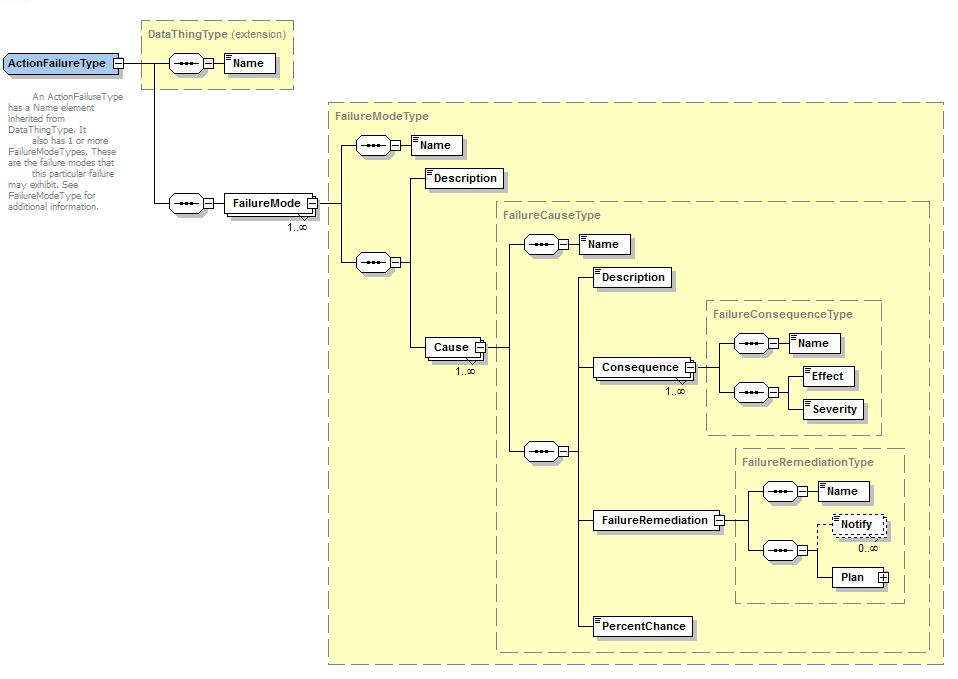
\includegraphics[width=12cm]{images/FailureType.jpg}
\caption{Description of the FailureType Class that is used to store information on action failures.}
\label{fig:failure}
\end{center}
\end{figure}
%
\section{Failure Analysis}
\label{sect:failure}
As seen in Figure~\ref{fig:predicateEval}, failures are identified during the evaluation of preconditions and effects. 
In addition to recognizing failures, it is desired to be able to respond to them.
In order to properly model this response, additional information must be modeled
in the ontology. As shown in Figure \ref{fig:failure}, the class {\it ActionFailureType} has been added to the ontology. This class is composed of a {\it PredicateType} class and a {\it FailureModeType} class. It contains all of the information required to be able to diagnose and remediate any failures that are detected by the system.

The {\it PredicateType} class contains a list of predicates whose truth values caused the detection of the current failure condition. Examination of the instances pointed to by the {\it ReferenceParameter} and the {\it TargetParameter} allow the system to understand exactly which components were involved in the failure.

The {\it FailureModeType} class provides various known failure modes that could exist for the combination of {\it PredicateType}s that were found deficient. It provides the consequences of such a failure occurring, information on how to remediate such a failure, and the chance that this kind of failure could occur. Understanding the consequences of the failure mode is important if one would like to be able to
pinpoint the correct cause of the failure. For example, assume that the action {\sc take-part} failed, and the predicate that indicated the failure was {\it part-location-robot}. 

Understanding where the part is actually located is critical to understanding the root cause of the failure. If the part is still in the parts tray, it would indicate a grasp related failure. If the part is on the floor of the cell, it would indicate a part handling error. This kind of information is represented in the {\it Effect} class of the consequences. Being able to pinpoint the effects of the failure also allows for judgment on the failure severity. A missed grasp will likely lead to a new grasp attempt and will have little impact on operation. A dropped part may cause damage to the part and have a higher severity level.

Failure remediation is described by the {\it FailureRemediation} class. This class contains information on what notifications need to be sent as a result of the failure as well as what actions should be taken. Continuing our example from above, the grasp failure may cause grasping information to be sent to the enginering department for algorithm refinement, while the dropped part may notify logistics that an additional component will be required. Recovery from the failure is possible by executing the {\it Plan} that accompanies the detected failure.

\section{Conclusions and Future Work}
\label{sect:future}
The framework described in this paper has been applied to the domain of kit building, which is a simple, but practically useful manufacturing/assembly domain. Through its use, we have been able to demonstrate agility in both kit construction through late binding of part locations, and in recovery from action failures through the detection of failures and ability to compensate for the failure's effects.

There are several areas in the system that still utilize hand-coding of data. It is desired that extensions to the ontology be created that will allow for the automatic application of knowledge and eliminate code that it specifically tuned to a particular set of predicates or actions. The hand-coded areas include the conversion of PDDL actions to CRCL sequences as well as the retrieval of instance data from the MySQL database for predicate evaluation. Work is currently underway to correct for these deficiencies. 

Extensions are also possible that will expand this work to the realm of general assembly. We hope to apply this knowledge based framework to simple assembly tasks (growing towards more complex tasks) on a real robot workcell in the near future. 

%
%



%
% ---- Bibliography ----
%
\bibliographystyle{plain}
\bibliography{rita2014}
\clearpage
\addtocmark[2]{Author Index} % additional numbered TOC entry
\renewcommand{\indexname}{Author Index}
\printindex
\clearpage
\addtocmark[2]{Subject Index} % additional numbered TOC entry
\markboth{Subject Index}{Subject Index}
\renewcommand{\indexname}{Subject Index}
%\input{subjidx.ind}
\end{document}
